\section{Effects on the extraction of the BAO scale}
\label{sec:BAO}
Having studied in the previous sections the effects of photo-z quality cuts on the measured galaxy auto- and cross-correlations and the way to correct for them, next we want to see how the extraction of the Baryon Acoustic Oscillations (BAO) scale from the measured galaxy auto-correlations in Fig.~\ref{auto_odcorr} is affected by the 
photo-z quality cuts and the subsequent correction. 

The BAO scale has been proven to be a successful standard ruler to constrain cosmological parameters \citep{Eisenstein2005, Hutsi2006, Percival2007, Padmanabhan2007, Okumura2008, Gaztanaga2009}. It was originated when primordial overdensities on matter caused acoustic (pressure) waves in the photon-baryon fluid that traveled freely across space until photons and baryons decoupled at the drag epoch (when the baryons were released from the ``Compton drag'' of the photons \citep{Hu1996}) $z_d=1059.25\pm0.58$ \citep{Ade2013}, and those waves stopped traveling. At that time, they had traveled $r_s(z_d)=147.49\pm0.59$~Mpc \citep{Ade2013} away from the primordial overdensities, where $r_s(z_d)$ is the sound horizon scale at the drag epoch. Later, when structure started forming, these waves seeded the formation of galaxies resulting in a small excess in the two-point angular galaxy correlation function at the correspondent angular scale: 
\begin{equation}
\theta_{BAO}(z) = r_s (z_d)/ r(z) \, ,
\label{bao_scale}
\end{equation}
where
\begin{equation}
r(z) = \int^z_0 {dz \over H_0\sqrt{\Omega_M(1+z)^3+\Omega_\Lambda}}
\label{comov_dist}
\end{equation}
is the comoving distance at redshift $z$ that only depends on the Hubble constant $H_0=67.3\pm1.2$~(km/s)/Mpc and the fraction of matter $\Omega_M=0.315^{+0.016}_{-0.018}$ \citep{Ade2013} in a flat $\Lambda$CDM cosmological model. In this case $\Omega_\Lambda = 1 - \Omega_M =0.685^{+0.018}_{-0.016}$. 

A first detection and measurement of the BAO scale $\theta_{BAO}$ in angular clustering was presented in~\citet{Carnero2012}. They made use of a method described in~\citet{Sanchez2011} that consists of fitting the empirical function
\begin{equation}
\omega(\theta) = A + B\theta^\gamma + Ce^{-(\theta-\theta_{FIT})^2 /2\sigma^2}
\label{bao_fit}
\end{equation}
to the observed angular correlation function in a range of angular separations that encloses the BAO peak, where $\lbrace A,B,\gamma,C,\theta_{FIT},\sigma \rbrace$ are the parameters of the fit. $A$ takes into account any possible global offset, $B$ and $\gamma$ describe the typical decreasing profile of $\omega(\theta)$, with $\gamma$ negative, and the rest is a Gaussian that characterizes the BAO peak. A non-zero value of $C$ will tell us that the BAO peak has been detected, $\theta_{FIT}$ is the location of that peak and $\sigma$ its width. Since angular correlations are measured in redshift bins of finite width due to the intrinsic photo-z dispersion, projection effects can cause a mismatch between $\theta_{FIT}$ and $\theta_{BAO}$. \citet{Sanchez2011} shows that this can be successfully corrected as follows:
\begin{equation}
\theta^{(obs)}_{BAO} = \alpha(z,\Delta z) \theta_{FIT} \, ,
\end{equation}
where $\alpha$ is a factor that only depends on the mean redshift $z$ and the width $\Delta z$ of the bin. Figure~3 in~\citet{Sanchez2011} shows these dependencies. In general terms, the wider the redshift bin, the larger the shift of $\theta_{FIT}$ towards smaller angles. For example, the shift is $\sim$5\% of $\theta_{BAO}$ when $\Delta z \sim 0.05$. For higher widths, only bins at $z\gtrsim0.5$ continue shifting, while the others saturate. 

In section~\ref{sec:photoz}, we chose a width of 0.05 for our photo-z bins in Fig.~\ref{Nz_bins}. This was in photo-z space. In real (spectroscopic) redshift space, this translates into a FWHM of $\sim$0.08, except in the last bin $0.6<z<0.65$ where, as a consequence of the poorer photo-z performance, the width becomes $\sim$0.12. We find that for those bins the shift in $\theta_{FIT}$ amounts to $\sim$7\%, except in the last bin, where it is $\sim$8\%.

Finally, we fit (\ref{bao_fit}) to the galaxy auto-correlation measurements of Fig.~\ref{auto_odcorr}. The results are shown on Fig.~\ref{bao_4bins}. Fits are performed in three different cases: when no photo-z quality cut and \textit{odds} correction are applied (black), when no photo-z quality cut is applied but the correction is (blue), and when the photo-z quality cut of 65\% completeness and the correction are applied (red). Error bars correspond to observations and are the same as in Fig.~\ref{auto_odcorr}. 
Solid and dashed lines correspond to the best fit, but in the dashed the BAO feature has been removed by setting $C=0$. The range of the fit is slightly changed in each photo-z bin to make sure that it completely encloses the BAO peak.
\begin{figure*}
\centering
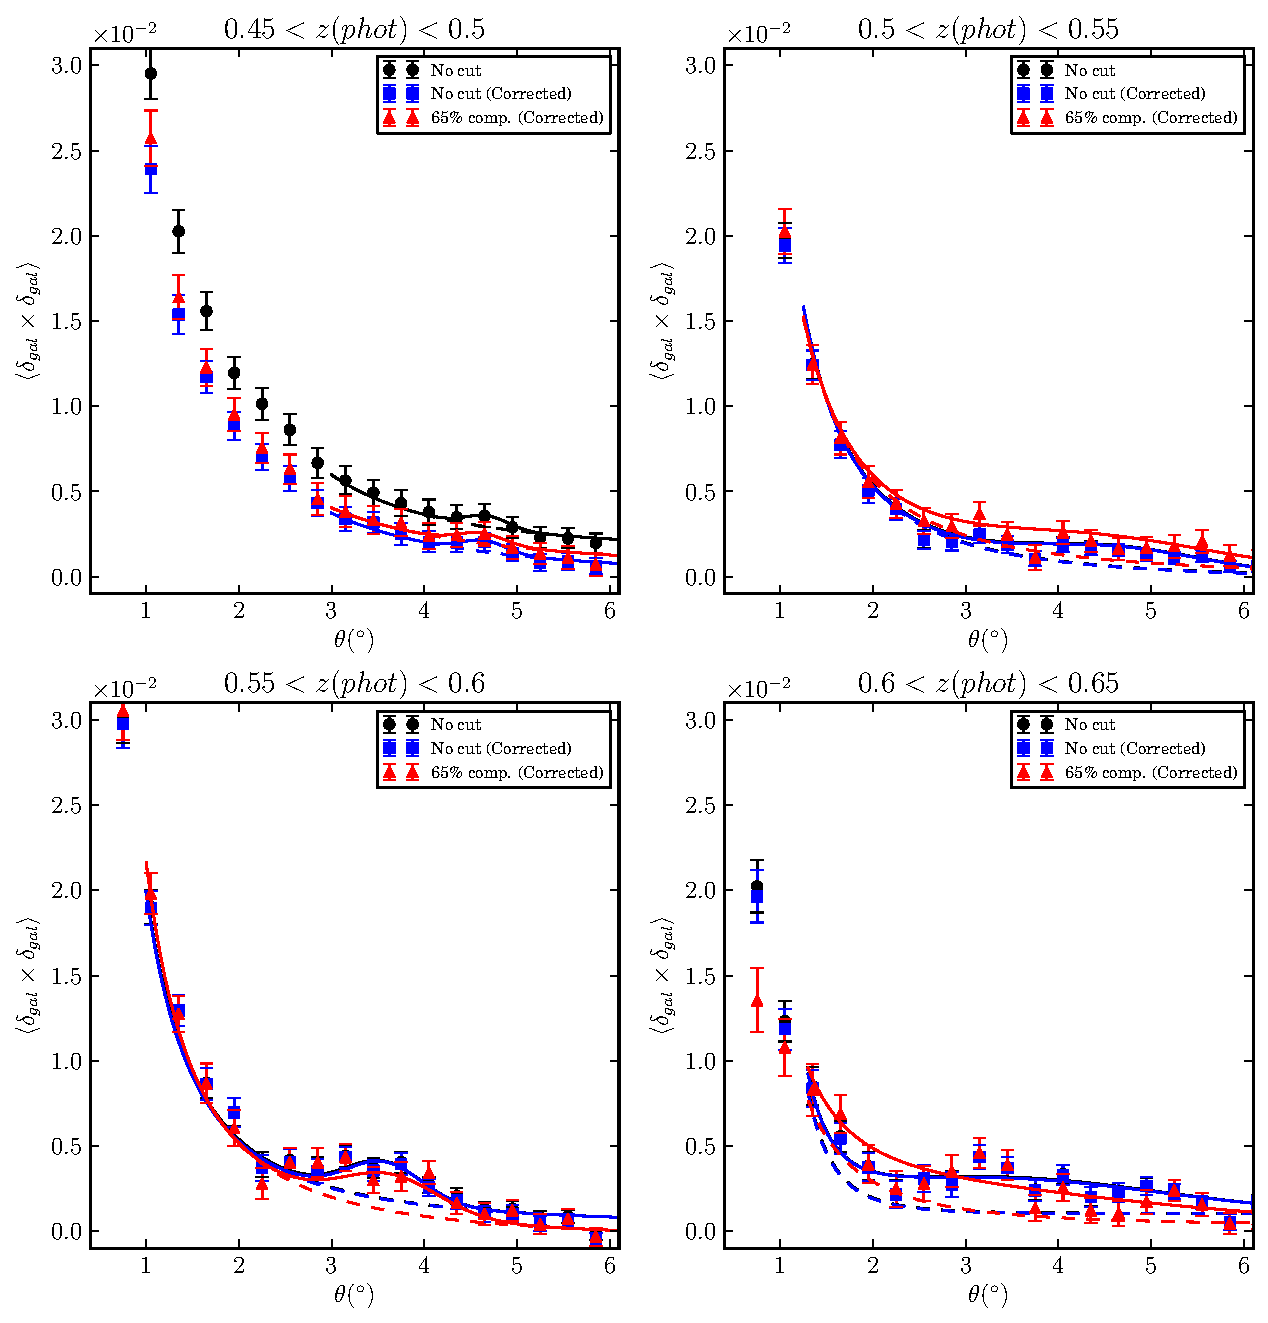
\includegraphics[type=pdf,ext=.pdf,read=.pdf, width=130mm]{./plots/bao_4bins_narrow}
\caption{Results of the fits of (\ref{bao_fit}) to the galaxy auto-correlations of Fig.~\ref{auto_odcorr} to extract the BAO scale. In black when no photo-z quality cut is applied, in blue the same but correcting for \textit{odds}, and in red when the 65\% completeness cut is applied and corrected. Error bars correspond to observations. Solid and dashed lines correspond both to the best fit, but in the dashed the BAO peak has been removed by setting $C=0$ in~(\ref{bao_fit}). 
}
\label{bao_4bins}
\end{figure*}
%

The results of the fits are summarized in Table~\ref{tab:BAO}. Looking at the parameter $C$, we see that we find evidence for the BAO peak (a non-zero value of $C$) in the first three bins, although with different significances in different bins. Typically, applying the photo-z quality cut and its correction (last column in Table~\ref{tab:BAO}) results in a decrease of the significance of the BAO peak, since 35\% of the galaxies are removed from the sample. The first and second column both correspond to the case in which no photo-z quality cut is applied. However, for the results in the second column the {\it odds} correction has been nevertheless applied using the formulas 
in~(\ref{od_correction}). This will correct for any intrinsic correlation between {\it odds} value and galaxy position that may create a spurious correlation in the galaxy map. Since higher {\it odds} may be due to larger signal-to-noise, the {\it odds} value may be seen as a proxy for airmass, seeing, extinction, etc. 
Therefore, it may make sense to correct for the {\it odds} effect even when applying no explicit {\it odds} cut in order to try to mitigate these effects. A comparison of the results in the second and third columns in Table~\ref{tab:BAO} shows that correcting for \textit{odds} when no cut is applied gives very similar results to simply not applying the correction. 
This is consistent with the findings in~\citet{Ho2012} and~\citet{Ross2011}, where they fail to see significant systematic effects in the galaxy auto-correlations due to differences in seeing, survey depth, extinction, etc. 

\begin{table*}
\caption{
Results of the BAO fits for the four photo-z bins, under three different conditions: no {\it odds} cut and no correction, no {\it odds} cut but correction for the {\it odds} effect, and finally after applying an {\it odds} cut that retains 65\% of the galaxies and the corresponding correction. The fit parameters are defined in Eq.~(\ref{bao_fit}). The rows labeled 
$\theta^{theo}_{BAO}$ contain the position of the BAO peak at the mean redshift in each bin derived from the latest Planck results~\citep{Ade2013}. The corresponding errors are derived by propagating the errors in the cosmological parameters in (\ref{bao_scale}) and (\ref{comov_dist}). Since the quality cut slightly changes the true redshift distribution inside each photo-z bin, the expected BAO scale in the bin may also change slightly.
} 
\vspace*{12pt}
\centering
\begin{tabular}{ c  c  c  c }
\cline{2-4} 
 & \parbox{3cm}{\centering No \textit{odds} cut} &  \parbox{3cm}{\centering No \textit{odds} cut\\+ Correction} & \parbox{3.5cm}{\centering \textit{Odds} cut (65\% eff.)\\+ Correction} \\ \cline{2-4}
\hhline{-===}
\multicolumn{4}{c}{$0.45<z<0.5$} \\ 
\hline
\multicolumn{1}{c}{C}& (0.7$\pm$0.3)$\cdot 10^{-3}$& (0.7$\pm$0.3)$\cdot 10^{-3}$& (0.6$\pm$0.4)$\cdot 10^{-3}$\\
\multicolumn{1}{c}{$\theta_{FIT}$}& 4.68$\pm$0.09& 4.65$\pm$0.09& 4.62$\pm$0.12\\
\multicolumn{1}{c}{$\theta^{obs}_{BAO}$}& 5.03$\pm$0.09& 5.00$\pm$0.08& 4.97$\pm$0.12\\
\multicolumn{1}{c}{$\theta^{theo}_{BAO}$}& 4.51$\pm$0.08& 4.51$\pm$0.08& 4.50$\pm$0.08\\
\hline
\hline
\multicolumn{4}{c}{$0.5<z<0.55$} \\ 
\hline
\multicolumn{1}{c}{C}& (1.2$\pm$0.4)$\cdot 10^{-3}$& (1.2$\pm$0.4)$\cdot 10^{-3}$& (1.5$\pm$0.6)$\cdot 10^{-3}$\\
\multicolumn{1}{c}{$\theta_{FIT}$}& 4.58$\pm$0.33& 4.59$\pm$0.32& 4.40$\pm$0.60\\
\multicolumn{1}{c}{$\theta^{obs}_{BAO}$}& 4.92$\pm$0.27& 4.94$\pm$0.27& 4.73$\pm$0.41\\
\multicolumn{1}{c}{$\theta^{theo}_{BAO}$}& 4.16$\pm$0.08& 4.16$\pm$0.08& 4.16$\pm$0.08\\
\hline
\hline
\multicolumn{4}{c}{$0.55<z<0.6$} \\ 
\hline
\multicolumn{1}{c}{C}& (2.2$\pm$0.4)$\cdot 10^{-3}$& (2.2$\pm$0.4)$\cdot 10^{-3}$& (2.2$\pm$0.6)$\cdot 10^{-3}$\\
\multicolumn{1}{c}{$\theta_{FIT}$}& 3.56$\pm$0.06& 3.57$\pm$0.06& 3.63$\pm$0.13\\
\multicolumn{1}{c}{$\theta^{obs}_{BAO}$}& 3.83$\pm$0.06& 3.84$\pm$0.06& 3.90$\pm$0.10\\
\multicolumn{1}{c}{$\theta^{theo}_{BAO}$}& 3.88$\pm$0.07& 3.88$\pm$0.07& 3.88$\pm$0.07\\
\hline
\hline
\multicolumn{4}{c}{$0.6<z<0.65$} \\ 
\hline
\multicolumn{1}{c}{C}& (2.1$\pm$0.5)$\cdot 10^{-3}$& (2.0$\pm$0.5)$\cdot 10^{-3}$& (2.0$\pm$4.4)$\cdot 10^{-3}$\\
\multicolumn{1}{c}{$\theta_{FIT}$}& 3.34$\pm$0.72& 3.30$\pm$0.77& 1.90$\pm$7.35\\
\multicolumn{1}{c}{$\theta^{obs}_{BAO}$}& 3.63$\pm$0.77& 3.59$\pm$0.81& 2.07$\pm$4.29\\
\multicolumn{1}{c}{$\theta^{theo}_{BAO}$}& 3.75$\pm$0.07& 3.75$\pm$0.07& 3.64$\pm$0.07\\
\hline
\end{tabular}
\label{tab:BAO}
\end{table*}

After applying the quality cut and its correction (last column), we recover values of $\theta^{obs}_{BAO}$ that are fully consistent with those found without applying an {\it odds} cut (first and second columns), demonstrating that our correction is consistent. In the last photo-z bin ($0.60 < z_{phot} < 0.65$), however,
the photo-z quality cut wipes out the BAO peak. We attribute this to the fact, already mentioned in section~\ref{sec:clustering}, that in this bin there are fewer galaxies than in the others, and even fewer after removing 35\% of them with the quality cut, and moreover, the photo-z performance is worse in this bin. 

It is worth mentioning that for some photo-z bins the theoretically-expected position of the BAO peak at the mean redshift in that photo-z bin, $\theta^{theo}_{BAO}$, changes slightly when the photo-z quality cut is applied. This is because $\theta^{theo}_{BAO}$ depends on $z$ (see Eq.~(\ref{bao_scale})) and, since the selection functions $N(z)$ change when quality cuts are applied, the mean redshift may also shift a little, shifting also $\theta_{BAO}$.  

We can see that in some bins there are some discrepancies between the extracted values of $\theta^{obs}_{BAO}$ and the expected $\theta^{theo}_{BAO}$. This is most likely due to systematic effects that lie beyond the scope of this thesis. The errors quoted in Table~\ref{tab:BAO} only contain the statistical uncertainties from the fit. In the two higher-redshift bins, where the BAO feature is detected with high statistical significance (over 4~$\sigma$), the observed BAO scales agree well with the expectations.  
In any case, the results of the fits are rather fragile, showing a significant dependence on details of the fits, such as the exact $\theta$ range chosen. Fits performed using the whole data covariance matrices (estimated with jack-knife) result in values for the $\chi^2$ per degree of freedom of order 2, signaling a poor fit quality. The same fits performed using only the diagonal elements of the covariance matrices result in very similar central values for $\theta_{FIT}$, but with larger errors and values of the $\chi^2$ per degree of freedom around 1. The main point of this section, however, can be qualitatively understood from looking only at the data points in Fig.~\ref{bao_4bins},  regardless of the fits: the position of the BAO peak does not change when going from data without {\em odds} cut and without correction to data without {\em odds} cut but with correction, and then to data with {\em odds} cut and with correction.

Finally, we have also tried to extract the BAO scale from the uncorrected auto-correlation functions after applying the most stringent {\em odds} cut. While in some bins, the fit has trouble converging, in those in which it does, the resulting BAO scale is only biased by a few percent, proving again the known fact that the BAO scale is very robust against systematic errors, even those, like this one, that grossly bias the overall shape and normalization of the correlation function. For example, in the bin with $0.55 < z < 0.60$, the BAO peak is found at $\theta^{obs}_{BAO} = (3.91 \pm 0.09)$~deg when applying the {\em odds} cut and no correction, to be compared with $\theta^{obs}_{BAO} = (3.90 \pm 0.10)$~deg, obtained applying the correction.

The main result of this section, however, is not another measurement of the BAO scale with the SDSS LRG sample, but rather the proof that after applying a tight photo-z quality cut that eliminates 35\% of the galaxies and severely distorts the shape of the galaxy-galaxy auto-correlation, the correction technique outlined in the previous section delivers a corrected auto-correlation function from which the BAO feature can be extracted without introducting any additional bias.
